\section{Lattice-based post-quantum cryptography} \label{post-quantum-cryptography-pqc}

\subsection{Lattices}
\subsubsection{Definitions}\label{lattice}
\begin{defn}
    Lattices in $\mathbb{R}^n$ are discrete subgroup of $\mathbb{R}^n$. Consider integer lattice $\mathcal{L}\subseteq \mathbb{Z}^n$, $\mathcal{L}$ can be represented by a basis $\mathbf{B}=[\mathbf{b}_1,\cdots,\mathbf{b}_n]\in\mathbb{Z}^{m\times n}$, where each vector $\mathbf{b}_i$ is written in column form as follow: 

$$\mathcal{L}(\mathbf{B}):=\left\{\sum_{i=1}^n\mathbf{b}_i x_i | x_i\in\mathbb{Z}~\forall i=1,\cdots,n \right\}\subseteq\mathbb{Z}^m.$$ 
\end{defn}

We refer to $n$ as the rank of the lattice $\mathcal{L}$ and $m$ as its dimension. $\mathcal{L}$ is called a full-rank lattice if $n=m$.

For a basis $\mathbf{B}$ of $\mathcal{L}$, we called $P(\mathbf{B})=\{\mathbf{B}\mathbf{x}|\mathbf{x}\in[0,1)^n\}$ is the fundamental parallelepiped of $\mathbf{B}$. A ``good'' basis of $\mathcal{L}$ results in a parallelepiped that is more square-like, whereas a ``bad'' basis produces a very thin parallelepiped. We denote$\|\mathbf{B}\|:=\max_{1 \le i \le k} \|\mathbf{b}_i\|$ the maximum $l_2$ length of the vectors in $\mathbf{B}$ and $\tilde{\mathbf{B}}:=\{\tilde{\mathbf{b}}_1,\cdots,\tilde{\mathbf{b}}_k \}$ the Gram-Schmidt orthogonalization of the vectors $\mathbf{b}_1,\cdots,\mathbf{b}_k$ in that order.


\begin{figure}[!htb]
	\centering
	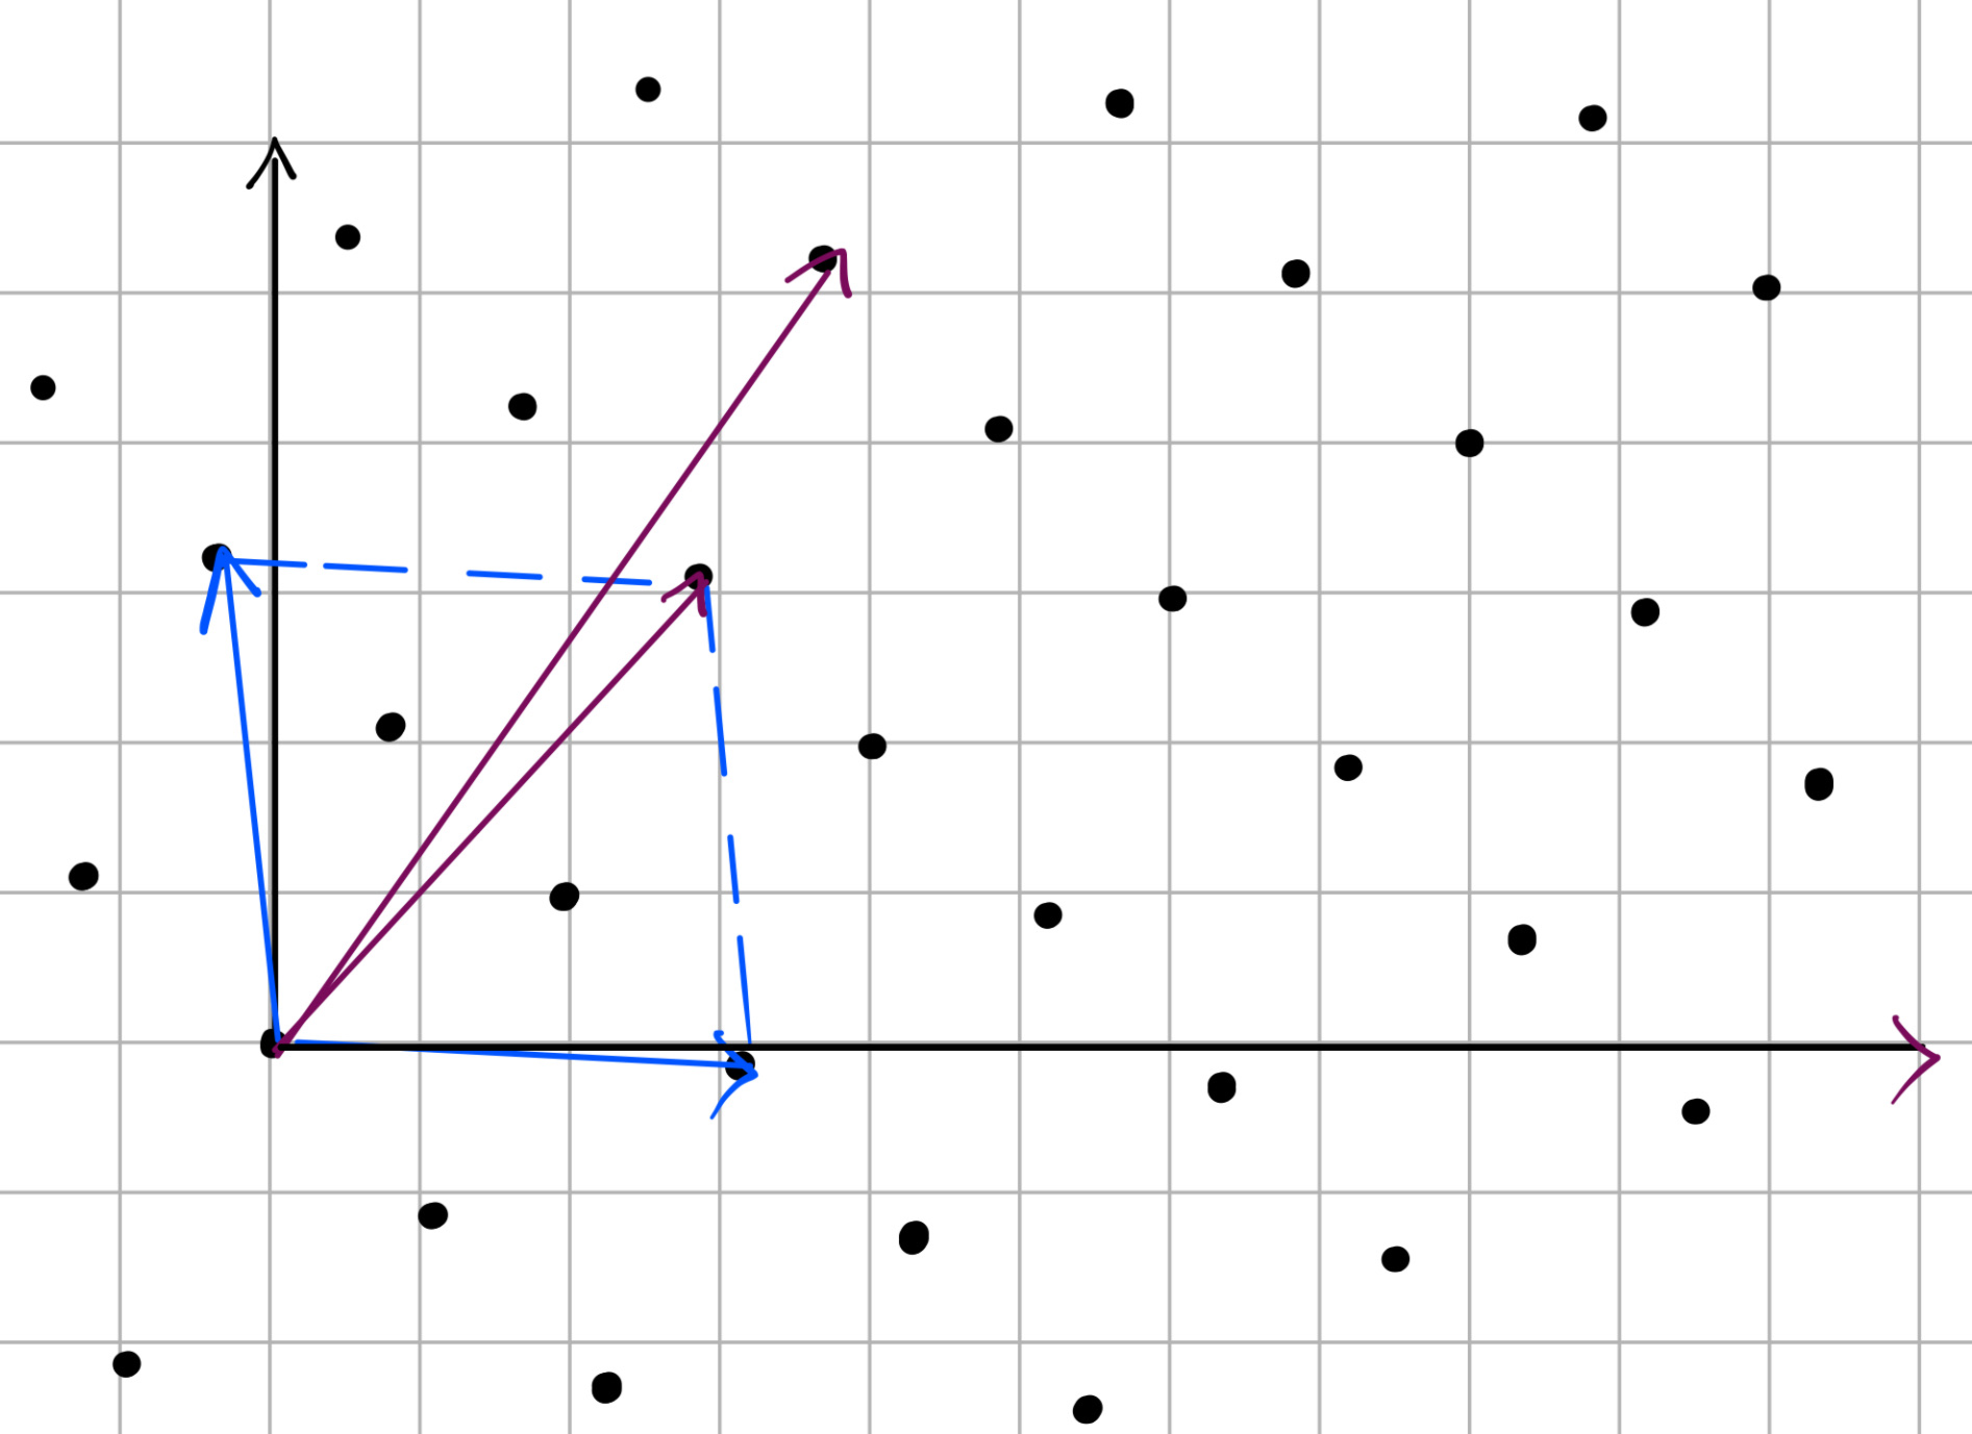
\includegraphics[scale=0.3]{figures/lattice_basis.pdf}
	\caption{Consider a two-dimensional lattice $\mathcal{L}$,  a basis for $\mathcal{L}$ consists of two non-zero vectors  $u$ and  $v$ such that any vector in $\mathcal{L}$ can be written as a linear combination of $u$ and $v$. A good basis for $\mathcal{L}$ will have vectors with lengths that are close to each other and an angle between them that is close to $90$ degrees.}\label{fig:lattice_basis}
\end{figure}

%\subsubsection{Hardness assumptions}

For a given lattice $\mathcal{L}(\mathbf{A})$, one basic parameter is the length of the shortest vector $\mathbf{s}$, denoted as $\lambda_1 = \|\mathbf{s}\|$ \peter{Here we should first define what \textbf{s} is}. This parameter is also called \textit{successive minima} if one considers the scenario where $\lambda_1$ is the smallest $r$ such that all the lattice points inside a ball of radius $r$ $\overline{\mathcal{B}}(0,r)$ span a space of dimension $1$. Similarly, we can define the $n^{th}$ successive minimum of $\mathcal{L}(\mathbf{A})$ as $\lambda_n(\mathcal{L}) = \inf\{r|\dim(\mathsf{span}(\mathcal{L}\cap \overline{\mathcal{B}}(0,r)))\leq n\}$.

%\textcolor{red}{Add an figure of sucessive minimum}

Hence, one of the most important problems in lattice-based cryptography is the Shortest Vector Problem ($\mathsf{SVP}$), which asks to find the shortest nonzero vector $\mathbf{s}$ in a given lattice $\mathcal{L}(\mathbf{A})$ with an arbitrary basis $\mathbf{A}$. There are also approximate versions of this problem called $\mathsf{SVP}_{\gamma}$ where the goal is to find a nonzero vector that is of length at most $\gamma = \gamma(n)\geq 1$ times the length of the optimal solution.

The ``decision'' versions of the problem ask to determine whether a given number $d$ is the minimum distance of $\mathcal{L}(\mathbf{A})$, i.e., $d = \min_{\mathbf{0}\neq \mathbf{v}\in\mathcal{L}}\|\mathbf{v}\|$.
This problem is known to be NP-hard in the $\ell_{\infty}$ norm, meaning there is no known polynomial-time algorithm to solve it~\cite{hardness_of_SVP}. For the $\ell_2$ (Euclid) norm, it remains a long-standing open problem. Another important problem is the Shortest Independent Vectors Problem ($\mathsf{SIVP}_{\gamma}$) with an approximation factor $\gamma$, a given a lattice $\mathcal{L}(\mathbf{A})$ with an arbitrary basis $\mathbf{A}$, $\mathsf{SIVP}_{\gamma}$ asks to find find $n$ linearly independent lattice vectors of length at most $\gamma(n)\cdot \lambda_{n}(\mathcal{L})$ where $\lambda_{n}(\mathcal{L})$ is the $n^{th}$ successive minimum of $\mathcal{L}$. Like $\mathsf{SVP}$, $\mathsf{SIVP}$ is also NP-hard.

\noindent Many hardness problems in lattice-based cryptography can be \textbf{``reduced''} to instances of $\mathsf{SVP}$ or $\mathsf{SIVP}$, for more information about reductions between lattice problems, please refer to~\ref{reduction} and ~\cite{reduction_lattice}.

\peter{The above intro on lattices we might expand upon to make it more accessible to a non-specialist audience.}

\subsubsection{Reductions}\label{reduction}

Within the realm of computational hardness challenges, the term ``reduction'' denotes a methodological approach whereby one problem is transformed into another, such that solving the second problem enables solving the first. This is a formal way to compare the intrinsic difficulty of different problems.  Specifically, if problem A can be reduced to problem B, and if one has a solution to B, then A can be solved. This doesn't necessarily imply that A is as hard as B, but that B is at least as hard as A. 

In the analysis of problem hardness, distinctions are made between \textit{worst-case} and \textit{average-case} scenarios. The \textit{worst-case} scenario is the most difficult possible instance for a given problem while the \textit{average-case} looks at the expected performance of an algorithm across all possible instances of a problem, usually under some reasonable assumption about the distribution of these instances. 

In Post-Quantum Cryptography (PQC), reductions are the main technique used to prove the security of cryptographic protocols by reducing their hardness to well-known hard problems. If such a reduction exists, then finding an efficient way to break the system would imply an efficient solution to the underlying hard problem, which is presumed not to exist, thus the security of the protocol holds.

%\textcolor{red}{Add an figure of reduction!!!!!! Can we illustrate reduction using some diagram?}


\subsection{SIS and LWE problems}
Let us first consider solving the linear equation
\begin{align}
    \mathbf{A}\mathbf{s} = \mathbf{y}\mod q \label{eq:linear_equation}
\end{align}

given $n,m \in \mathbb{Z}$, a prime number $q$, a matrix $\mathbf{A}$ in $\mathbb{Z}^{m\times n}_q$ and $\mathbf{y}$ is a vector in $\mathbb{Z}^m_q$. 

We can now view the matrix $\mathbf{A}$ as a basis for a lattice $\mathcal{L}(\mathbf{A})$. Note that solving Eq.~\eqref{eq:linear_equation} is achievable through Gaussian elimination. However, its variations, along with many other related lattice problems, are known to be NP-hard (based on the factors of polynomial approximation problems). Here, we highlight some significant lattice problems: \textbf{The shortest integer solution (SIS)} and \textbf{The Learning With Errors (LWE)} problems, further information on lattice-related problems can be found in~\cite{Pei16}.

\subsubsection{The shortest integer solution (SIS)}

Recall that initially, we are attempting to find a solution for the equation $\mathbf{A}\mathbf{s} = \mathbf{y} \mod q$. Consider an additional constraint that $\mathbf{s}$ is ``short'', i.e $\mathbf{s}$ lies in the subset $S=\{0,1\}^n\in\mathbb{Z}^n_q$; or more generally, $S=[-B,\dots, B]^n$  ($B\ll q/2$). Since we are seeking a \textit{short solution} to linear equations, this problem is referred to as the \textit{Short Integer Solution} (SIS) problem. Many cryptographic protocol deal with the case $\mathbf{y}=\mathbf{0}$, the $\mathbf{SIS}_{n,m,q,B}$ problem can be stated as follows:

\begin{defn}
    Let $n,m,q, B \in \mathbb{N}$ be positive integers. Given a uniformly sampled matrix $\mathbf{A}\in\mathbb{Z}^{n\times m}_q$, the shortest integer solution problem asks to find a none zero vector $\mathbf{s}\in\mathbb{Z}^m_q$ such that $\mathbf{A}\mathbf{s}=\mathbf{0}\mod q$ and $\|x\|_{\infty}\leq B$.
\end{defn}

One should think of $n$ as the security parameter that defines the hardness of the problem (the bigger $n$ is, the harder the problem becomes), $m$ usually depends on the specific application, generally $m\gg n$, $q=poly(n)$ and $B$ should be set large enough to ensure that a solution exists, but not trivial to solve. It is proven that solving the $\mathbf{SIS}_{n,m,q, B}$ problem is at least as hard as solving the $\mathsf{SVP}_{\gamma}$ on worst-case $n$-dimensional lattices with high probability for some approximation factor $\gamma$~\cite{Pei16}.


\subsubsection{The learning with errors problem (LWE)}
This subsection recalls the definition of the Learning With Errors (LWE) problem~\cite{Pei16}. Let's revisit Eq.~\eqref{eq:linear_equation}, we can consider a slight variant of it where the input pair $(\mathbf{A}\in \mathbb{Z}^{m\times n}_q, \mathbf{y} \in \mathbb{Z}^m)$ satisfies
\begin{align}
    \mathbf{A}\mathbf{s} + \mathbf{e}= \mathbf{y}\mod q \label{eq:lwe}
\end{align}
where $n, m, q$ are positive integers and $\mathbf{e}$ is an additional small noise term sample from an error distribution $\chi$ over $\mathbb{Z}^n$. 

The ``search'' $\mathsf{LWE}_{n,m,q,\chi}$ problem asks to find $\mathbf{s}\in\mathbb{Z}^n$ and the ``decision'' version asks to to distinguish between the distribution $ (\mathbf{A},\mathbf{y}=\mathbf{A}\mathbf{s}+\mathbf{e} \mod q)$ and a uniformly random sample $(\overline{\mathbf{A}},\mathbf{u})$.

The error term $\mathbf{e}$ effectively affects the exact relationship between the secret $\mathbf{s}$ and $\mathbf{y}$. Specifically, this term $\mathbf{e}$ ensures that although anyone can observe the pairs $(\mathbf{A},\mathbf{y})$, extracting the information of $\mathbf{s}$ is computationally infeasible if the problem is properly parameterized. The hardness of the $\mathsf{LWE}_{n,m,q,\chi}$ problem (and thus the security of many $\mathsf{LWE}$-based cryptosystems) relies on the assumption that finding $\mathbf{s}$ with random errors is as difficult as solving certain worst-case problems on lattices, more information is mentioned in~\ref{reduction}.

\subsubsection{Distribution over lattices}
It's important to note that the choice of the error distribution $\chi$ is crucial. A widely utilized distribution in numerous lattice-based cryptosystems is the Discrete Gaussian distribution. Typically, the discrete Gaussian is chosen in a way that ensures the errors $\mathbf{e}$ are small enough to allow for the correct extraction of the secret information but large enough to prevent adversaries from solving the problem.


For any positive integer $n$ and real $\sigma>0$, which is taken to be $1$ when omitted, the \textit{Gaussian function} $\rho_{\sigma}:\mathbb{R}^n\to \mathbb{R}^+$ of parameter (or width) $\sigma$ is defined 
\begin{align}
    \rho_{\sigma}(\mathbf{s}):=\exp(-\pi\|\mathbf{s}|\|^2/\sigma^2).
\end{align}

A \textbf{discrete Gaussian probability distribution} $D_{\mathcal{L},\sigma}$ over a lattice $\mathcal{L}$ is given by
\begin{align}
    D_{\mathcal{L},\sigma}(\mathbf{s})=\displaystyle{\frac{\rho_{\sigma}(\mathbf{s})}{\rho_{\sigma}{\mathcal{L}}}}, \forall \mathbf{s}\in\mathcal{L}.
\end{align}


The utilization of Gaussian distributions comes from its ability to effectively connect the Learning With Errors (LWE) problem to the worst-case scenario of the lattice NP-hard problems, thus providing a solid foundation for cryptographic security.

More concretely, a long sequence of works has established progressively stronger results about the worst-case lattice problems. It is shown that for any $\alpha>0$ such that $\sigma=\alpha q \geq 2\sqrt{n}$, the $\mathsf{LWE}_{n,m,q, D_{\mathbb{Z}_q,\sigma}}$, where $D_{\mathbb{Z}_q,\sigma}$ is the discrete Gaussian distribution, is at least as hard as approximating the shortest independent vector problem $(\mathsf{SIVP}_{\gamma})$ to within a factor of $\gamma = \Tilde{O}(n/\alpha)$~\cite{Reg09,RPS17}.

%For a lattice $\mathcal{L}$ and $\epsilon>0$, the smoothing parameter $\eta_{\epsilon}(\mathcal{L})$ of $\mathcal{L}$ is the smallest number $s$ satisfied $\rho_{1/\sigma}(\mathcal{L}^*\setminus \{0\})\leq \epsilon$.


%\begin{lem} For a lattice $\mathcal{L}$, a vector $\mathbf{c}\in\mathbb{R}^n$, $\epsilon>0$ and $\sigma\geq \eta_{\epsilon}(\mathcal{L})$, the statistical distance between $D_{\sigma}+\mathbf{c}\mod \mathcal{L}$ and the uniform distribution $\mathbb{R}^n/\mathcal{L}$ is at most $\epsilon/2$.\end{lem}


\subsubsection{Trapdoor mechanism}

In cryptography, a \textbf{trapdoor} refers to a concealed backdoor embedded within an algorithm or a specific piece of data. The idea is that, except for the individuals authorized to hold the trapdoor, others cannot extract any information about the trapdoor. This characteristic enables secure communication between parties. This subsection revisits certain trapdoor mechanisms to provide a fundamental understanding of the relationship between lattices and their trapdoors.

The first approach to constructing trapdoors for lattices involves the use of short bases, as these lead to more efficient algorithms for solving lattice problems. Algorithms designed to tackle challenges such as the Shortest Vector Problem (SVP) or the Closest Vector Problem (CVP) become more practical with basis vectors that are short and nearly orthogonal~\ref{lattice}. This is because the computations involved are simpler and can be executed more swiftly. Specifically, for solving the LWE problem using a short basis, one strategy employs Babai's nearest plane algorithm~\cite{Babai}. The initial step involves utilizing a short basis $\mathbf{T}_{\mathbf{A}}$ of a lattice $\mathcal{L}(\mathbf{A})$ to identify the lattice vector closest to $\mathbf{y}$. Given that the error is sufficiently ``small'', it becomes feasible to extract the secret vector $\mathbf{s}$'s information. A sequence of works has been carried out to develop more trapdoor mechanisms. Two of the notable approaches are~\cite{AP09} and~\cite{MP12}.

\cite{AP09} presented an algorithm to sample a uniform matrix $\mathbf{A}\in\mathbb{Z}_q^{n\times m}$ together with an associated basis $\mathbf{T}$ of $\mathcal{L}({\mathbf{A}})$ with a low Gram-Schmidt norm such that $\mathbf{A}\mathbf{T}_{\mathbf{A}} = \mathbf{0}$ as the public matrix and its secret trapdoor. The second approach is the trapdoor technique from~\cite{MP12}, which we focus on more due to its simpler, more elegant nature, and its support for more efficient cryptographic constructions.

\cite{MP12} first defined a ``primitive vector'' $\mathbf{g}=\{g_1,\dots,g_k\}\in\mathbb{Z}^k_q$ where $\gcd(g_1,\dots,g_k,q)=1$. Then
a matrix $\mathbf{G}\in\mathbb{Z}^{n\times m}_q$ is called ``primitive matrix'' if its columns generate all of $\mathbb{Z}^n_q$, i.e., $\mathbf{G}\mathbb{Z}^m=\mathbb{Z}^n_q$. We can now define the $\mathbf{G}$-trapdoor of a lattice $\mathcal{L}$ is a matrix $\mathbf{R}\in\mathbb{Z}^{(m-\omega)\times \omega}$ such that $\mathbf{A}\begin{pmatrix}
    \mathbf{R}\\ 
    \mathbf{I}
  \end{pmatrix} = \mathbf{H}\mathbf{G}$ for some invertible matrix $\mathbf{H}\in\mathbb{Z}^{n\times n}_q$. We refer to $\mathbf{H}$ as the \textbf{tag} or \textbf{label} of the trapdoor. 

The paper also presented an efficient algorithm $\mathsf{GenTrap}(1^n,1^m,q)$ that returns a matrix $\mathbf{A}\in\mathbb{Z}^{n\times m}_q$ and a trapdoor $\mathbf{T}_{\mathbf{A}}=\mathbf{R}$ such that the distribution of $\mathbf{A}$ is negligibly (in $n$) close to the uniform distribution. 

Moreover, there is an efficient algorithm $\mathsf{Invert}$ that, on input $\mathbf{A}$, $t_{\mathbf{A}}$ and $\mathbf{A}\mathbf{s}+\mathbf{y}$ where $\mathbf{s}\in\mathbb{Z}^n_q$ is arbitrary and $\mathbf{y}\gets \mathcal{D}_{\mathbb{Z}^m,\alpha q}$ for $1/\alpha \geq \sqrt{n\log q}\cdot \omega(\sqrt{\log n})$, outputs $\mathbf{s}$ and $\mathbf{y}$ with overwhelming probability over $(\mathbf{A},\mathbf{t}_{\mathbf{A}})\gets \mathsf{GenTrap}(1^n,1^m,q)$. By using the ``strong'' trapdoor $\mathbf{R}$, one also can efficiently generate the ``weak'' trapdoor $\mathbf{T}_{\mathbf{A}}$ or $\mathbf{s}$. Since in lattice-based PQC, these trapdoors $\mathbf{R},\mathbf{T}_{\mathbf{A}}, \mathbf{s}$ can be used as the secret keys of hierarchical parties in some hierarchical cryptosystems.

\peter{The above we could also expand to make more accessible.}

\subsection{RLWE problem}

There is a variant of the LWE problem that has been widely used in recent years called the Ring Learning With Error problem (RLWE). The primary benefit of using polynomial rings in RLWE offer more efficient and practical implementations of cryptographic schemes with significantly smaller keys and signature sizes while maintaining strong security guarantees.

Here, let's first recall some basic ideas of the RLWE problem.

\subsubsection{The initial idea.}
Let's recall that the SIS problem in Eq.~\eqref{eq:linear_equation} yields a very simple collision-resistant hash function that is provably secure if worst-case lattice problems are hard:
\begin{align}
    h_{\mathbf{A}}(\mathbf{s})=\mathbf{A}\mathbf{s} \mod q
\end{align}
where $\mathbf{A}\in\mathbb{Z}^{m\times n}_q$ is uniformly random and $\mathbf{s}\in \{0,1\}^n$. 

However, this is inefficient, since just reading the public description of $\mathbf{A}$ takes time roughly $mn\log q>n^2$. The goal is now to show a variant of $h_{\mathbf{A}}$ whose running time is roughly linear in $n$. 

A trivial idea is taking some short, uniformly random seed $r$ and then setting $\mathbf{A} = H(\textsf{seed})$ for some suitable expanding function $H$. However, we need to describe $H$ so that it can be efficiently used in cryptography constructions. 


Let's first take the random seed to be $\ell = m/n$ uniformly random vectors $\mathbf{a}_1,\dots,\bf{a_{\ell}}\in[q]^n$. Consider the ``cyclic rotations'' of $\mathbf{a}_i$, i.e. for a single vector $\mathbf{a}=(a_1,\dots,a_n)^T\in\mathbb{Z}^n$, we define
\begin{align}
    \mathsf{Rot}(\mathbf{a})=
    \begin{pmatrix}
    a_1 & a_n &\dots& a_3 & a_2\\
    a_2 & a_n &\dots& a_4 & a_3\\
    a_3 & a_n &\dots& a_5 & a_4\\
    \vdots & \vdots &\ddots& \vdots & \vdots\\
    a_{n-2} & a_{n-3} &\dots& a_n & a_{n-1}\\
    a_{n-1} & a_{n-2} &\dots& a_1 & a_n\\
    a_{n} & a_{n-1} &\dots& a_2 & a_1
    \end{pmatrix}\in\mathbb{Z}^{n\times n},
\end{align}
    where each column is a simple cyclic permutation of the previous column. 
    %Matrices of the form $\mathsf{Rot}(\mathbf{a})$ are sometimes called \textit{cyclic matrices}. 
    $\mathbf{A}$ can now be rewritten as
\begin{align}
    \mathbf{A}=
    \begin{pmatrix}
    \mathsf{Rot}(\mathbf{a}_1)\\
    \mathsf{Rot}(\mathbf{a}_2)\\
    \vdots\\
    \mathsf{Rot}(\mathbf{a}_{\ell})
    \end{pmatrix}\in\mathbb{Z}^{m\times n}.
\end{align}

\noindent Due to the property of $\mathsf{Rot}(\mathbf{a}$, we can write $\mathsf{Rot}(\mathbf{a})=(\mathbf{a}),\bf{X}\mathbf{a},\dots,X^{n-1}\mathbf{a})$ 
where 
\begin{align}
    \bf{X}=
    \begin{pmatrix}
    0 & 0 &\dots& 0 & 1\\
    1 & 0 &\dots& 0 & 0\\
    0 & 1 &\dots& 0 & 0\\
    \vdots & \vdots &\ddots& \vdots & \vdots\\
    0 & 0 &\dots& 1 & 0
    \end{pmatrix}\in\{0,1\}^{n\times n}
\end{align}
    is the ``cyclic shift'' matrix. 
   
\noindent Consider the set of all integer cyclic matrices, $\Tilde{R}:=\{\mathsf{Rot}(\mathbf{a}):\mathbf{a}\in\mathbb{Z}^n\}$. Hence we have that $\Tilde{R}$ is a lattice with rank $n$ and basis $\{\bf{I}_n,\bf{X},\bf{X}^2,\dots,\bf{X}^{n-1}\}$. We have that $\tilde{R}$ is a commutative ring. We can instead think of $\mathsf{Rot}(\mathbf{a})\in\tilde{R}$ as the corresponding polynomial $a\in R=\mathbb{Z}[x]/(x^n-1)$. Hence, we can therefore identify the matrix $\mathbf{A}\in\mathbb{Z}_q^{m \times n}$ with a tuple of ring elements $(a_1,\dots,a_{\ell})^T\in R^{\ell}_q= R=\mathbb{Z}^{\ell}_q[x]/(x^n-1)$. Similarly, $\mathbf{s}$ is a tuple of ring elements $(s_1,\dots,s_{\ell})^T\in R^{\ell}_{\{0,1\}}$.
    Therefore, $h_{\mathbf{A}}$ can be written as 
\begin{align}
    h_a(s)=h_{a_1,\dots,a_{\ell}}(s_1,\dots,s_{\ell})=a_1s_1+\dots+s_{\ell}s_{\ell}\mod qR.
\end{align}
     The Ring-SIS problem, which is the analogue of SIS in this setting, can be defined as follows: For a ring $R$, integer modulus $q\geq 2$, and integer $\ell\geq 1$. Given $a_1,\dots, a_{\ell}\in R_q$ sampled independently and uniformly at random. The search Ring-SIS problem asks to output $e_1,\dots e_{\ell}\in R_{\{-1,0,1\}}$ not all zero such that $h_{a_1,\dots,a_{\ell}}(e_1,\dots,e_{\ell})=a_1e_1+\dots+a_{\ell}e_{\ell} = 0\mod qR$.


    However, for security reasons, there exist attacks on $h_a$ over $\mathbb{Z}[x]/(x^n-1)$ since $(x^n-1)$ has a nontrivial factor over the integers. So, it is natural to try replacing $(x^n-1)$ with an irreducible polynomial $p(x)$. 


    If $n$ is a power of $2$, we have that $x^n+1$ is an irreducible polynomial and $R=\mathbb{Z}[x]/(x^n+1)$ is an integral domain. From the matrix perspective mentioned above, this corresponds to taking
\begin{align}
    \mathsf{Rot}(\mathbf{a})=
    \begin{pmatrix}
    a_1 & -a_n &\dots& -a_3 & -a_2\\
    a_2 & a_n &\dots& -a_4 & -a_3\\
    a_3 & a_n &\dots& -a_5 & -a_4\\
    \vdots & \vdots &\ddots& \vdots & \vdots\\
    a_{n-2} & a_{n-3} &\dots& -a_n & -a_{n-1}\\
    a_{n-1} & a_{n-2} &\dots& -a_1 & -a_n\\
    a_{n} & a_{n-1} &\dots& a_2 & a_1
    \end{pmatrix}\in\mathbb{Z}^{n\times n},
\end{align}
    and 
\begin{align}
    \bf{X}=
    \begin{pmatrix}
    0 & 0 &\dots& 0 & -1\\
    1 & 0 &\dots& 0 & 0\\
    0 & 1 &\dots& 0 & 0\\
    \vdots & \vdots &\ddots& \vdots & \vdots\\
    0 & 0 &\dots& 1 & 0
    \end{pmatrix}\in\{-1,0,1\}^{n\times n}.
\end{align}
    Matrices of the form $\mathsf{Rot}(\mathbf{a})$ as above are occasionally called ``\textit{anti-cyclic}''. Ring-SIS is hard over this ring, under a reasonable worst-case complexity assumption.

\subsubsection{Ideal lattices and computational problems}
Recall that a lattice is an additive subgroup of $\mathbb{Z}^n$,i.e., a subset of $\mathbb{Z}^n$ closed under addition and subtraction. An ideal $\mathcal{I}\subset R=\mathbb{Z}[x]/(x^n+1)$ is an additive subgroup of $R$ that is closed under multiplication by any ring element. Concretely, $\mathcal{I}$ is closed under addition and subtraction, and for any $y\in\mathcal{Y}$ and $r\in R$, we have that $ry\in\mathcal{I}$.

For the choice of ring, we can view $\mathcal{I}$ as a lattice by embedding $R$ in $\mathbb{Z}^n$ via the trivial embedding that maps $x_i$ to the unit vector $\mathbf{e}_i$. We have that $\mathcal{I}\subset \mathbb{Z}^n$ is a lattice such that $(y_1,\dots,y_n)^T \in \mathcal{I}$ if and only if $(-y_n,y_1\dots,y_{n-1})^T \in \mathcal{I}$. Such lattices are sometimes called ``anti-cyclic" lattices.\\
This view of ideals as lattices is useful since we can extend computational lattice problems to ideals. Concretely, for some fixed ring $R$, we can define the computational problems IdealSVP, IdealSIVP, GapIdealSVP, etc., similar to SVP, SIVP, etc. as the corresponding computational problems restricted to ideal lattices.

\subsubsection{The Ring-LWE problem}
Here we define the Ring-LWE in a similarly natural way as the Ring-SIS problem.

For integers $q\geq 2$, a power of two $n$, and an error distribution $\chi$ over short elements in $R_q = \mathbb{Z}_q[x]/(x^n+1)$, the (average-case, search) Ring-LWE problem (RLWE) is defined as follows: 
Given $a_1,\dots, a_{m}\in R_q$ sampled independently and uniformly at random together with $b_1,\dots,b_{m}\in R_q$ where $b_i=a_i s + e_i \mod R_q$ for $s\in R_q$, and $e_i\gets \chi$, find $s$.



\subsubsection{Trapdoor algorithms in the ring setting}

The trapdoor mechanism techniques from~\cite{MP12} can be generalised to the ring setting where there exists an efficient randomised algorithm $\mathsf{GenTrap}(1^n,1^m,q)$ that returns $\mathbf{a}=(a_1,\dots,a_m)\in R^{m}_q$ and a trapdoor $t_{\mathbf{a}}$ such that the distribution of $\mathbf{a}$ is negligibly (in $n$) close to the uniform distribution. Moreover, there is an efficient algorithm $\mathsf{Invert}$ and a universal constant $C_T$ that, on input $\mathbf{a}$, $t_{\mathbf{a}}$ and $\mathbf{a}\cdot s+\mathbf{e}$ where $s \in R_q$ is arbitrary and $\|\mathbf{e}\|\leq q/(C_T\sqrt{n\log q})$, outputs $s$ with overwhelming probability.
